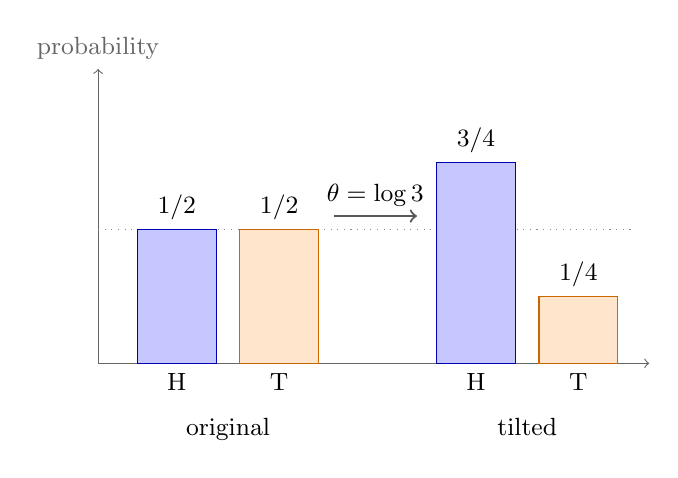
\begin{tikzpicture}[x=1cm,y=3.4cm]
\draw[->,black!60] (0,0)--(7,0);
\draw[->,black!60] (0,0)--(0,1.1) node[above,font=\small] {probability};
\draw[dotted,black!45] (0,0.5)--(6.8,0.5);
\draw[fill=blue!22,draw=blue!70!black] (0.5,0) rectangle (1.5,0.5);
\draw[fill=orange!20,draw=orange!80!black] (1.8,0) rectangle (2.8,0.5);
\draw[fill=blue!22,draw=blue!70!black] (4.3,0) rectangle (5.3,0.75);
\draw[fill=orange!20,draw=orange!80!black] (5.6,0) rectangle (6.6,0.25);
\node[above,font=\small] at (1,0.5) {$1/2$};
\node[above,font=\small] at (2.3,0.5) {$1/2$};
\node[above,font=\small] at (4.8,0.75) {$3/4$};
\node[above,font=\small] at (6.1,0.25) {$1/4$};
\foreach \x/\lab in {1/H,2.3/T,4.8/H,6.1/T}{\node[below,font=\small] at (\x,0) {\lab};}
\draw[->,thick,black!65] (3,0.55)--(4.05,0.55);
\node[above,font=\small] at (3.52,0.55) {$\theta=\log3$};
\node[below,font=\small] at (1.65,-0.17) {original};
\node[below,font=\small] at (5.45,-0.17) {tilted};
\end{tikzpicture}
